Every software development process has a starting point, but saying that it has an end point can be ambiguous. Once the software is deployed in a production environment and all \glspl{feature} have been developed, it can be assumed that the development phase is complete and the end point has been reached. At this point, software maintenance, often referred to as software support, can begin and additional system \glspl{enhancement} can be made. Maintenance usually focuses on \gls{bug} fixes or new \glspl{enhancement}, but sometimes end users may request \glspl{feature} that require additional development, which restarts the development process 

Given the cyclical nature of software processes, numerous software process models \cite{pavlic2009is} have been developed by various authors throughout history. The most famous model, the waterfall model, was introduced in the 1970s, but did not address the cyclic nature of software processes and was therefore an inefficient mechanism for software development. Over time, other models were developed to improve the rigidity of the waterfall model, leaving a variety of options to choose from to select the most appropriate software process model and create a flexible \acrlong{sdlc}. 

A software process model is used to identify the system to be built. It defines the activities for designing, implementing, testing, and monitoring software systems. Some software process models include the classic Waterfall Model, Incremental and Iterative Models and their combination, the \acrfull{rad} Model, various Prototyping Models, the Spiral model, the \acrfull{rup} Model, the V-model (verification and validation model) as an extended implementation of the Waterfall Model, and others \cite{pi2019}. The waterfall model is a precursor to other software process models, but it poses risks to the project outcome due to its linear (sequential) life cycle model.

All the models listed have similarities between the phases they define (analysis, design, development, test, and maintenance). Most models are based on an iterative life cycle model that allows for flexible requirements updates, and they are often user-driven in an \gls{agile} manner. The \gls{data-platform} created as part of this thesis is a small project guided by an implementation of iterative rapid prototyping through Analysis, Design, and Development \& Testing cycles.


\begin{center}
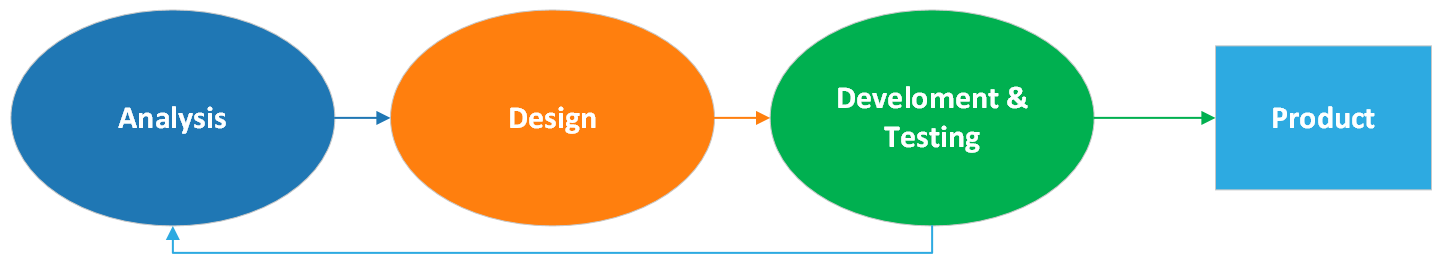
\includegraphics[width=14cm,keepaspectratio]{images/twitter-data-platform-sdlc.png}
\label{figure:twitter-data-platform-sdlc}
\captionof{figure}{Twitter \Gls{data-platform} \acrshort{sdlc}}
\end{center}

During Development \& Prototype, there was frequent switching between the analysis phase and the development and testing phase. This model has proven to be a fast development and release process, especially for features that required additional testing 

After the Testing phase demonstrates that the developed system meets the requirements of the Development \& Prototype phase, the Maintenance phase is initiated. This transition requires that data output not be compromised by developers, analysts, or others interacting with the \gls{data-platform}, so a production environment is introduced. This means that development and testing must occur as infrequently as possible and with as few changes as possible to avoid \gls{data-integrity} issues. To improve the security of the system, native GitHub functions such as \gls{branch-protection-rules} can be used.

The following subsections describe the rapid prototyping phases in the platform life cycle.

\vspace{1.2cm}
\subsubsection{Analysis}
\label{subsec:sdlc-analysis}
% \setlength\parindent{0pt}

The \textbf{goal} of this thesis is to create a dataset that provides valuable knowledge about the information being shared on Twitter and to enable analyzing social trends on Twitter through time.

Analysis phase identifies the \textbf{\gls{data-service-provider}}, \textbf{data source} endpoints, their limitations and restrictions, and finally - \textbf{data requirements}.

\paragraph{\Gls{data-service-provider}} Twitter\footnote{https://twitter.com} is the \gls{data-service-provider} for this \gls{data-platform}. The provided \acrshort{rest} service imposes various limitations and restrictions, some of them being \underline{Tweet limits} - \textit{up to 500k Tweets} are served per month and \underline{User limits} - \textit{inability to lookup Users} in a given range (location, age...). The identified limitations and restrictions need to be accounted for at the earliest stages of the Analysis phase. Failing to do so may result with disastrous effects on the product at a stage when it is too late to iterate over Analysis again. This \gls{data-platform} accounts for \underline{Tweet limits} with an option of creating multiple accounts if the \textit{500k Tweets per month} limit is surpassed and re-running the full load process (\ref{sec:methods-data-ingestion}). \underline{User limits} are accounted for by creating a baseline list of User IDs and \textit{}{expanding} it with each \gls{data-pipeline} run \textit{}{using the user's followers and friends IDs} \cite{mipro2022c19prediction}.

\paragraph{Data source} Data source endpoints are used to collect information about Twitter defined User objects and Tweet objects. Endpoints impose technical limitations, with most common limitations including a limited number of \acrshort{api} requests that an external system can make to the data source's \acrshort{rest} server. These limitations are documented in table \ref{tables:source-endpoints-limitations}.

\begin{table}[ht]
	\centering
	\begin{tabular}{ | p{4.2cm} | p{5.7cm} | p{2.6cm} | }
		\hline \textbf{Name}  & \textbf{Description}   & \textbf{Limitations} \\
		\hline
		\hline \href{https://developer.twitter.com/en/docs/twitter-api/v1/accounts-and-users/follow-search-get-users/api-reference/get-users-lookup}{users/lookup}\footnote{https://developer.twitter.com/en/docs/twitter-api/v1/accounts-and-users/follow-search-get-users/api-reference/get-users-lookup} & serves \glspl{user-object} & 900 requests / 15 minutes \\
		\hline \href{https://developer.twitter.com/en/docs/twitter-api/v1/tweets/timelines/api-reference/get-statuses-user_timeline}{statuses/user\_timeline}\footnote{https://developer.twitter.com/en/docs/twitter-api/v1/tweets/timelines/api-reference/get-statuses-user\_timeline} & serves \glspl{tweet-object} associated with a user & 900 requests / 15 minutes \\
		\hline \href{https://developer.twitter.com/en/docs/twitter-api/v1/accounts-and-users/follow-search-get-users/api-reference/get-followers-ids}{followers/ids}\footnote{https://developer.twitter.com/en/docs/twitter-api/v1/accounts-and-users/follow-search-get-users/api-reference/get-followers-ids} & serves user's follower IDs  & 15 requests / 15 minutes \\
		\hline \href{https://developer.twitter.com/en/docs/twitter-api/v1/accounts-and-users/follow-search-get-users/api-reference/get-friends-ids}{friends/ids}\footnote{https://developer.twitter.com/en/docs/twitter-api/v1/accounts-and-users/follow-search-get-users/api-reference/get-friends-ids} & serves user's friends IDs & 15 requests / 15 minutes \\
		\hline

	\end{tabular}
    \caption{Source data Endpoints Descriptions \& Limitations}
\end{table}
\label{tables:source-endpoints-limitations}

\paragraph{Data requirements} Data requirements identify the information that needs to be obtained from the data source. The \gls{data-service-provider} must be capable of satisfying the given data requirements by providing curated sets of information. The resulting \gls{data-platform} must be designed to support the given data requirements. The following bullet list provides the requirements summary:

\begin{itemize}
    \item \textbf{Users quantity}: Croatian users only
    \item \textbf{Tweets quantity}: from \texttt{2022-11-01} onward
    \item \textbf{Data re-usability}: never delete ingested data
    \item \textbf{Object details}: identify attributes that can be used to analyse social trends
\end{itemize}

Collected (\textit{ingested} afterwards) data needs to provide as much information about \textit{data source} objects as possible. This is accomplished by storing all available source object attributes and only eliminating irrelevant attributes in the \nameref{sec:methods-data-transformation} process. The ingested data is never deleted, moved or modified (in place).

The following paragraphs describes some valuable \textit{data source} object attributes and other inputs used to apply User and Tweets quantitative restrictions.

\paragraph{Location Inputs} A User object is identified as a Croatian user if their \texttt{location} attribute \textbf{contains} at least one Croatian location from \ref{methods:sdlc-inputs-locations}. As an example, if a User object's \texttt{location} attribute is set to \texttt{"Zaprešić"}, he will be identified as a Croatian user because (\texttt{"Zaprešić"} is a subset of \texttt{"Zaprešić,Croatia"} \textbf{or} \texttt{"Zaprešić,Croatia"} is a subset of \texttt{"Zaprešić"}). 


\begin{code}
\captionof{listing}{Croatian Locations Input} 
\label{methods:sdlc-inputs-locations}
\begin{minted}[frame=single,
               framesep=3mm,
               tabsize=2]{js}
[
    "Hrvatska",
    "Croatia",
    "Žminj",
    "Zaprešić,Croatia",
    "Virovitica",
    "republic of dalmatia baby!",
    "velika gorica, croatia",
    "RIJEKA"
]
\end{minted}
\end{code}

The \nameref{methods:sdlc-inputs-locations} was derived manually by inspecting the \nameref{subsubsec:sdlc-analysis-data-source:ingest-user}'s \texttt{location} attribute values and capturing them in a separate \acrshort{json} file. The values were only inspected once and the input locations were not revised since. 

Additional transformations were performed on \nameref{methods:sdlc-inputs-locations} to ensure Users are correctly identified as Croatian users. Some transformations include converting the \texttt{location} strings to lowercase, punctuation and diacritics removal and white-space and Unicode character removal. 

These operations were simple to execute on this input file, but they were time-expensive when applied to the User models and they did not yield results that would justify their use. After performing this due diligence, the additional transformation functionality was discarded and it is no longer in use.



\paragraph{Ingested Users} The User object contains a large number of attributes. Only a subset of attributes are presented and described, but all of them are ingested. Details about all attributes can be found at the Twitter's \href{https://developer.twitter.com/en/docs/twitter-api/v1/data-dictionary/object-model/user}{Tweet object}\footnote{https://developer.twitter.com/en/docs/twitter-api/v1/data-dictionary/object-model/user} page.

\clearpage
\begin{code}
\captionof{listing}{Ingest User}
\label{subsubsec:sdlc-analysis-data-source:ingest-user}
\begin{minted}[frame=single,
               framesep=3mm,
               tabsize=2]{js}
{
    "name": "HNS",
    "screen_name": "HNS_CFF",
    "location": "Hrvatska | Croatia",
    "description": "Službeni Twitter profil Hrvatskog"
                   "nogometnog saveza Croatian Football"
                   "Federation official Twitter feed."
                   "#HNS #Obitelj #Family",
    "protected": false,
    "followers_count": 262456,
    "friends_count": 116,
    "statuses_count": 19515
}
\end{minted}
\end{code}

\begin{itemize}
    \item \texttt{name}: The name of the user, as they have defined it. Not necessarily a person's name
    \item \texttt{screen\_name}: The screen name, handle, or alias that this user identifies themselves with. \texttt{screen\_names} are unique but subject to change
    \item \texttt{location}: \textit{Nullable}. The user-defined location for this account's profile
    \item \texttt{description}: \textit{Nullable}. The user-defined UTF-8 string describing their account
    \item \texttt{protected}: When true, indicates that this user has chosen to protect their Tweets (\href{https://help.twitter.com/en/managing-your-account/about-twitter-verified-accounts}{Verified Accounts}\footnote{https://help.twitter.com/en/managing-your-account/about-twitter-verified-accounts})
    \item \texttt{followers\_count}: The number of followers this account currently has
    \item \texttt{friends\_count}: Number of accounts that the user follows
    \item \texttt{statuses\_count}: The number of users this account is following (also known as their \texttt{"followings"})
\end{itemize}


\clearpage
\paragraph{Ingested Tweets} Twitter uses the term \textit{status} when referring to a Tweet. The Tweet object contains a large number of attributes. Only a subset of attributes are presented and described, but the entire set is ingested. Details about all attributes can be found at the Twitter's \href{https://developer.twitter.com/en/docs/twitter-api/v1/data-dictionary/object-model/tweet}{Tweet object}\footnote{https://developer.twitter.com/en/docs/twitter-api/v1/data-dictionary/object-model/tweet} page.

\begin{code}
\captionof{listing}{Ingest Tweet}
\label{subsubsec:sdlc-analysis-data-source:ingest-tweet}
\begin{minted}[frame=single,
               framesep=3mm,
               tabsize=2]{js}
{
    "created_at": "Tue Nov 22 10:00:18 +0000 2022",
    "full_text": "VATRENI IS LISTED"
                 "\n\nThis is truly a historic moment"
                 "because #VATRENI is so much more "
                 "than just a token. Become a part"
                 "of the greatest fan story and enjoy"
                 "all kinds of benefits.\n\n#VATRENI"
                 "token is now live at @gate_io \n\n",
    "entities": {
        "hashtags": [
            {"text": "VATRENI"},
            {"text": "VATRENI"}
        ],
        "user_mentions": [
            {"id": 912539722, "screen_name": "gate_io"}
        ]
    },
    "user": { ingested_user },
    "retweet_status": { ingested_tweet },
    "in_reply_to_status_id": null,
    "in_reply_to_user_id": null,
    "quoted_status": { ingested_tweet },
    "favorite_count": 41,
    "possibly_sensitive": false,
    "lang": "en"
}
\end{minted}
\end{code}

\begin{itemize}
    \item \texttt{created\_at}: UTC time when this Tweet was created
    \item \texttt{full\_text}: The actual UTF-8 text of the status update
    \item \texttt{entities}: Entities which have been parsed out of the text of the Tweet. Additionally see \href{https://developer.twitter.com/overview/api/entities-in-twitter-objects}{Entities in Twitter objects}\footnote{https://developer.twitter.com/overview/api/entities-in-twitter-objects}
        \begin{itemize}
        \item \texttt{hashtags}: Names of the hashtags used in this Tweet, minus the leading \texttt{"\#"} character
        \item \texttt{user\_mentions}: IDs of the mentioned users, as an integer
        \end{itemize}
    \item \texttt{user}: Ingested User (\nameref{subsubsec:sdlc-analysis-data-source:ingest-user})
    \item \texttt{retweet\_status}: Retweets can be distinguished from typical Tweets by the existence of a retweeted\_status attribute. This attribute contains a representation of the original Tweet that was retweeted (\nameref{subsubsec:sdlc-analysis-data-source:ingest-tweet})
    \item \texttt{in\_reply\_to\_status\_id}: \textit{Nullable}. If the represented Tweet is a reply, this field will contain the integer representation of the original Tweet's ID
    \item \texttt{in\_reply\_to\_user\_id}: \textit{Nullable}. If the represented Tweet is a reply, this field will contain the integer representation of the original Tweet's author ID
    \item \texttt{is\_quote\_status}: Indicates whether this is a Quoted Tweet
    \item \texttt{quoted\_status}: This attribute contains a representation of the original Tweet that was quoted (\nameref{subsubsec:sdlc-analysis-data-source:ingest-tweet}). Quote tweets are Retweets that contain some original content (\texttt{full\_text}, \texttt{hashtagas}, \texttt{user\_mentions})  
    \item \texttt{favorite\_count}: \textit{Nullable}. Indicates approximately how many times this Tweet has been liked by Twitter users
    \item \texttt{possibly\_sensitive}: \textit{Nullable}. This field indicates content may be recognized as sensitive. This may also be judged and labeled by an internal Twitter support agent
    \item \texttt{lang}: \textit{Nullable}. When present, indicates a \href{http://tools.ietf.org/html/bcp47}{BCP 47}\footnote{http://tools.ietf.org/html/bcp47} language identifier corresponding to the machine-detected language of the Tweet text, or und if no language could be detected
\end{itemize}



\clearpage
\subsubsection{Design}
\label{subsec:sdlc-design}

Design phase focuses on shaping the mechanisms by which data is ingested and transformed to create a dataset that can be easily used for data analysis 

The resulting \gls{data-platform} must support storage of the full raw data as-is, without any changes being made in the ingestion process (\ref{sec:methods-data-ingestion}). The transformation process uses the full data set to apply filters and changes to the raw data. This process performs read operations on the ingested data, transforms \gls{in-memory} data, and stores the resulting dataset in a new location that is independent of the ingestion location. Before the resulting dataset is stored, it is filtered to contain only Croatian users, and the baseline list of User IDs is overwritten with the available Croatian user IDs. Figure \ref{figure:twitter-data-platform-design} shows an overview of the implemented \gls{data-platform} architecture.

\begin{center}
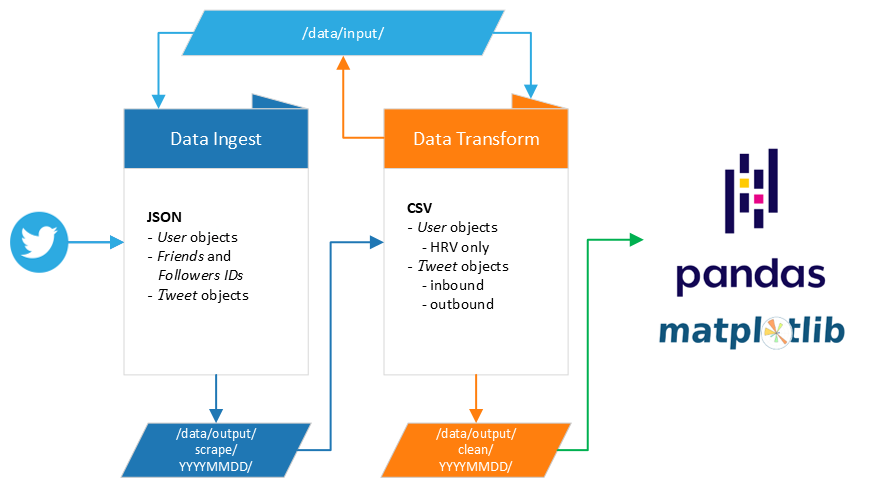
\includegraphics[width=14cm,keepaspectratio]{images/twitter-data-platform.png}
\label{figure:twitter-data-platform-design}
\captionof{figure}{Twitter \Gls{data-platform} Architecture}
\end{center}

Both ingestion and transformation output locations (in particular, the directories reflecting the ingestion date) are created at runtime. This mechanism allows the ingested and transformed data to be examined per ingestion date, and ensures that only the most recently ingested data is transformed, rather than the entire data for each \gls{data-pipeline} run. The resulting dataset is a union of all files in the date directories in the output file system of the data conversion and is analysed (\ref{sec:methods-data-analysis}) using the \gls{pandas} and \gls{matplotlib} tools.

\paragraph{Data target filesystem} A filesystem is used to store data throughout the \gls{data-pipeline}. The data is stored on an on-premise Linux server provided by the University of Rijeka. The filesystem includes two main directories: \texttt{input} and \texttt{output}. The \texttt{output} directory is then divided into the \texttt{scrape} ( ingested data) and \texttt{clean} (transformed data) directories, partitioned by date.
\vspace{0.6cm}
\begin{figure}[hb]
\dirtree{%
.0 data.
    .1 input.
        .2 locations.
            .3 hr.json.
    .1 output.
        .2 scrape.
            .3 tweets.
                .4 2022-11-01.
            .3 users.
                .4 ids.
                    .5 2022-11-01.
                .4 objs.
                    .5 2022-11-01.
        .2 clean.
            .3 tweets.
                .4 2022-11-01.
            .3 users.
                .4 2022-11-01.
}
\caption{Data target file system structure}
\end{figure}
\label{tabels:target_fs}


\vspace{1.2cm}
\subsubsection{Development \& Testing}
\label{subsec:sdlc-development}

Development (Prototyping) \& Testing phase is focused on developing the mechanisms used to ingest, and transform data defined in the \nameref{subsec:sdlc-design} phase. This phase ensures that ingestion and transformation are independent (\gls{loosely-coupled}) processes, that enable historical and incremental data ingestion, notification mechanism and CI/CD mechanisms (\ref{sec:methods-cicd}).


\vspace{1.2cm}
\subsubsection{Maintenance}
\label{subsec:sdlc-maintenance}

Maintenance phase focuses on supporting the end-users in their \gls{data-platform} usage. Once Development \& Testing is completed and the system is deployed to \textit{production}, it is maintained to ensure that any unexpected \glspl{bug} are promptly fixed and supported to accommodate new \glspl{enhancement}. This phase may also support \gls{feature} development requests, but if a development effort exceeds the scope of the defined Design, a new iteration is initiated across \acrshort{sdlc} phases.
